\pagebreak

\section*{Q6}
\begin{solution}
\hfill\break
Code is given after. Here we produce the same solution curves using two approximate methods and we can compare it to our exact method from Q5.
\begin{figure}[H]
    \centering
    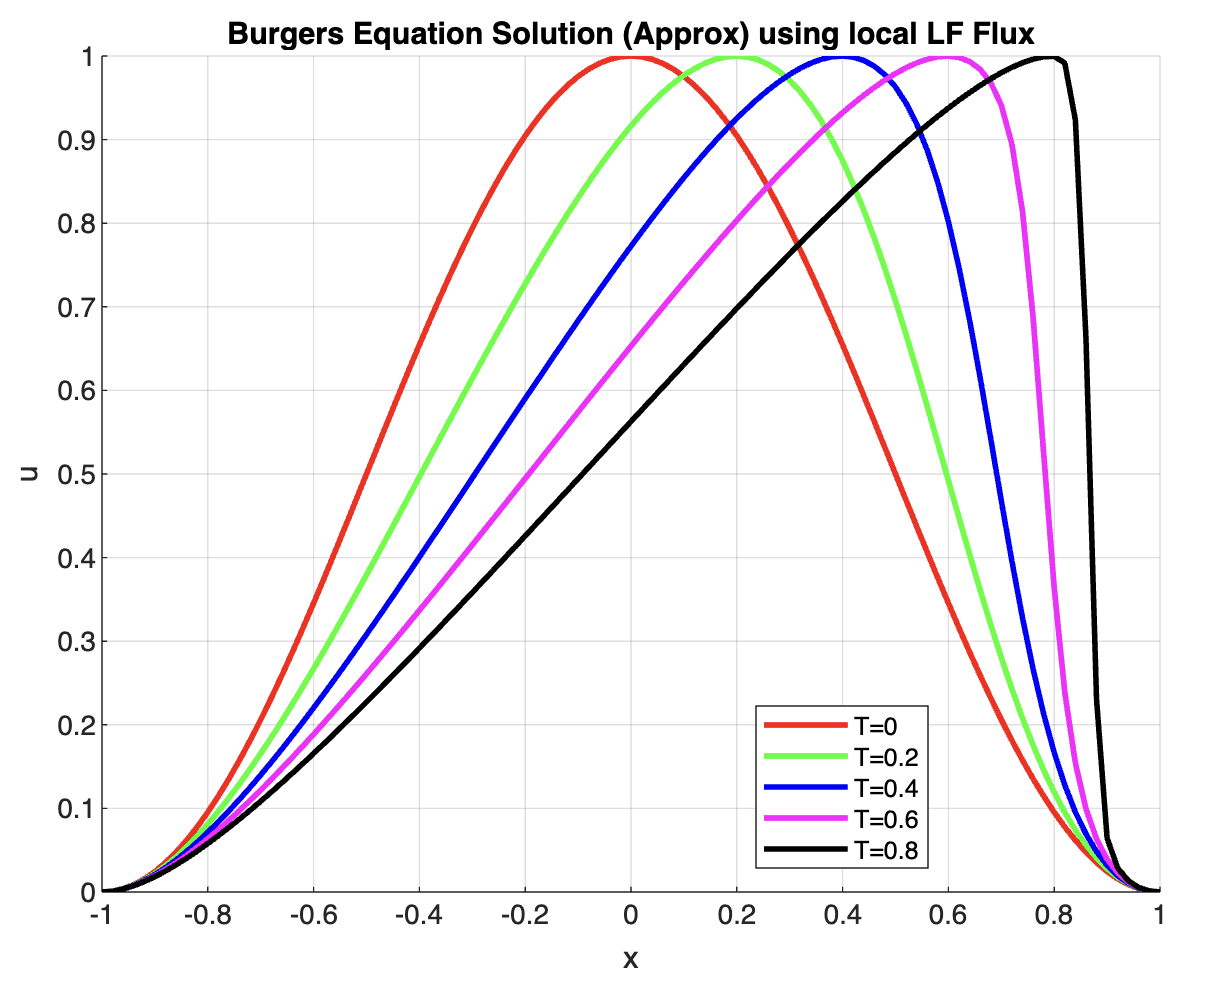
\includegraphics[scale=0.4]{./figures/q6-cos-local.png}
    \caption{Solving the Burgers equation with a local flux approximate method and cosine initial condition.}
\end{figure}
\begin{figure}[H]
    \centering
    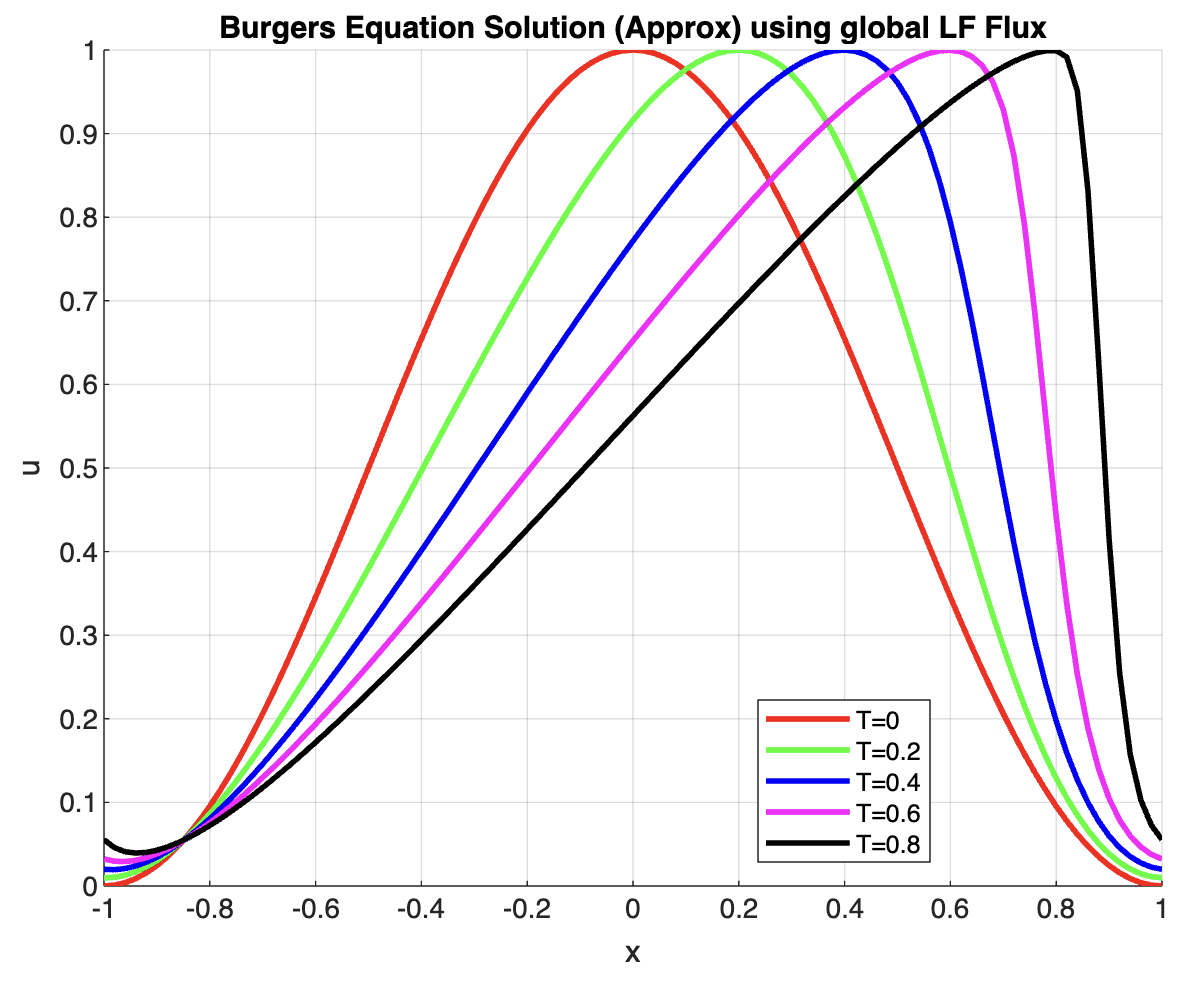
\includegraphics[scale=0.4]{./figures/q6-cos-global.png}
    \caption{Solving the Burgers equation with a global flux approximate method and cosine initial conditions.}
\end{figure}
\begin{figure}[H]
    \centering
    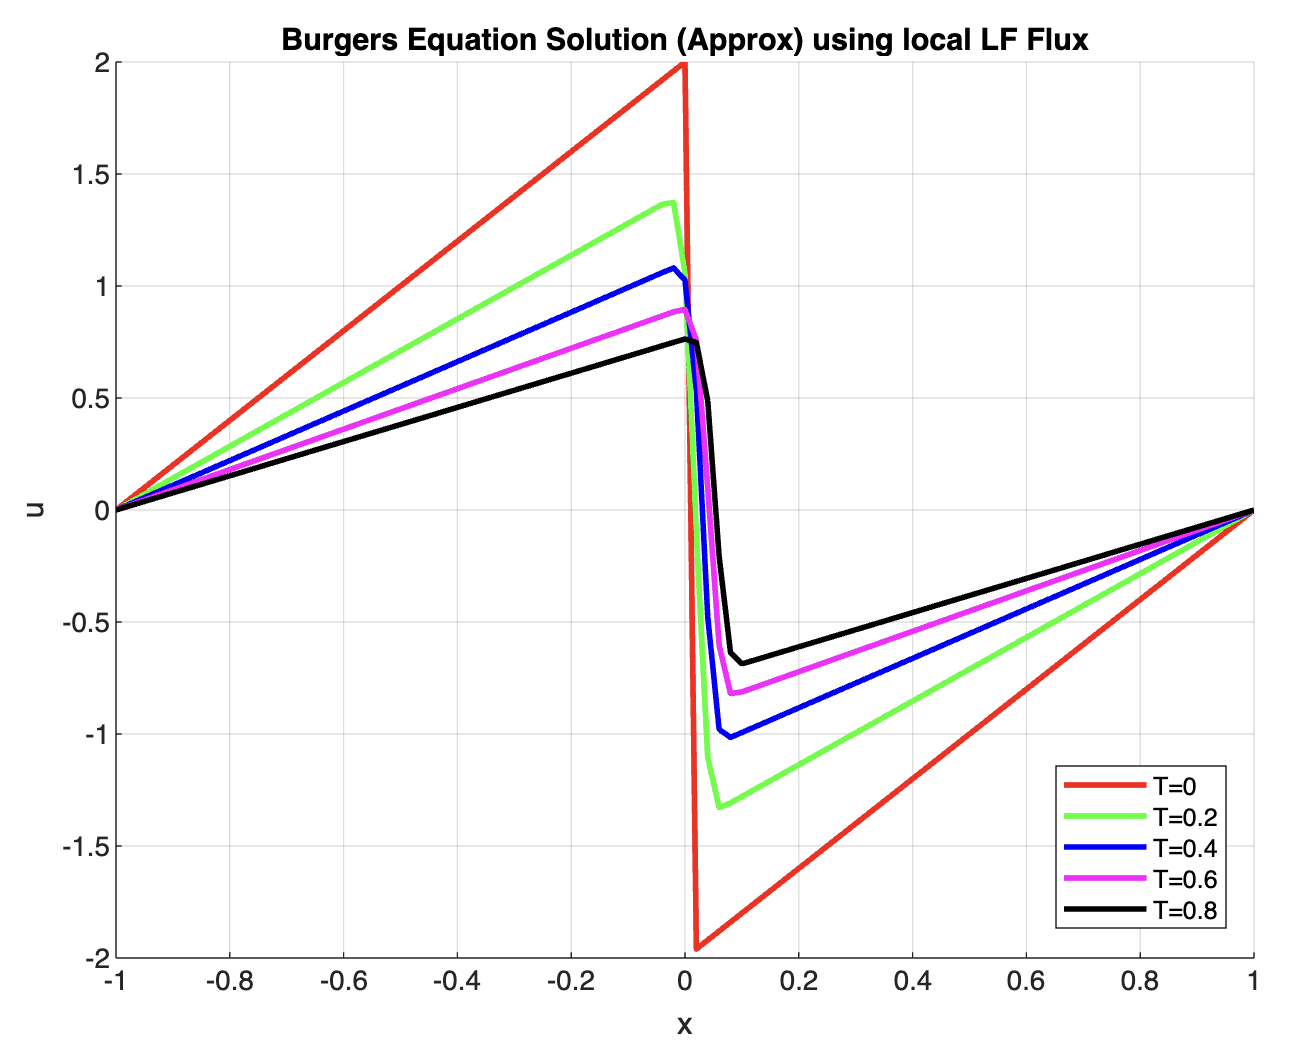
\includegraphics[scale=0.4]{./figures/q6-triangular-local.png}
    \caption{Solving the Burgers equation with a global flux approximate method and triangular initial conditions.}
\end{figure}
\begin{figure}[H]
    \centering
    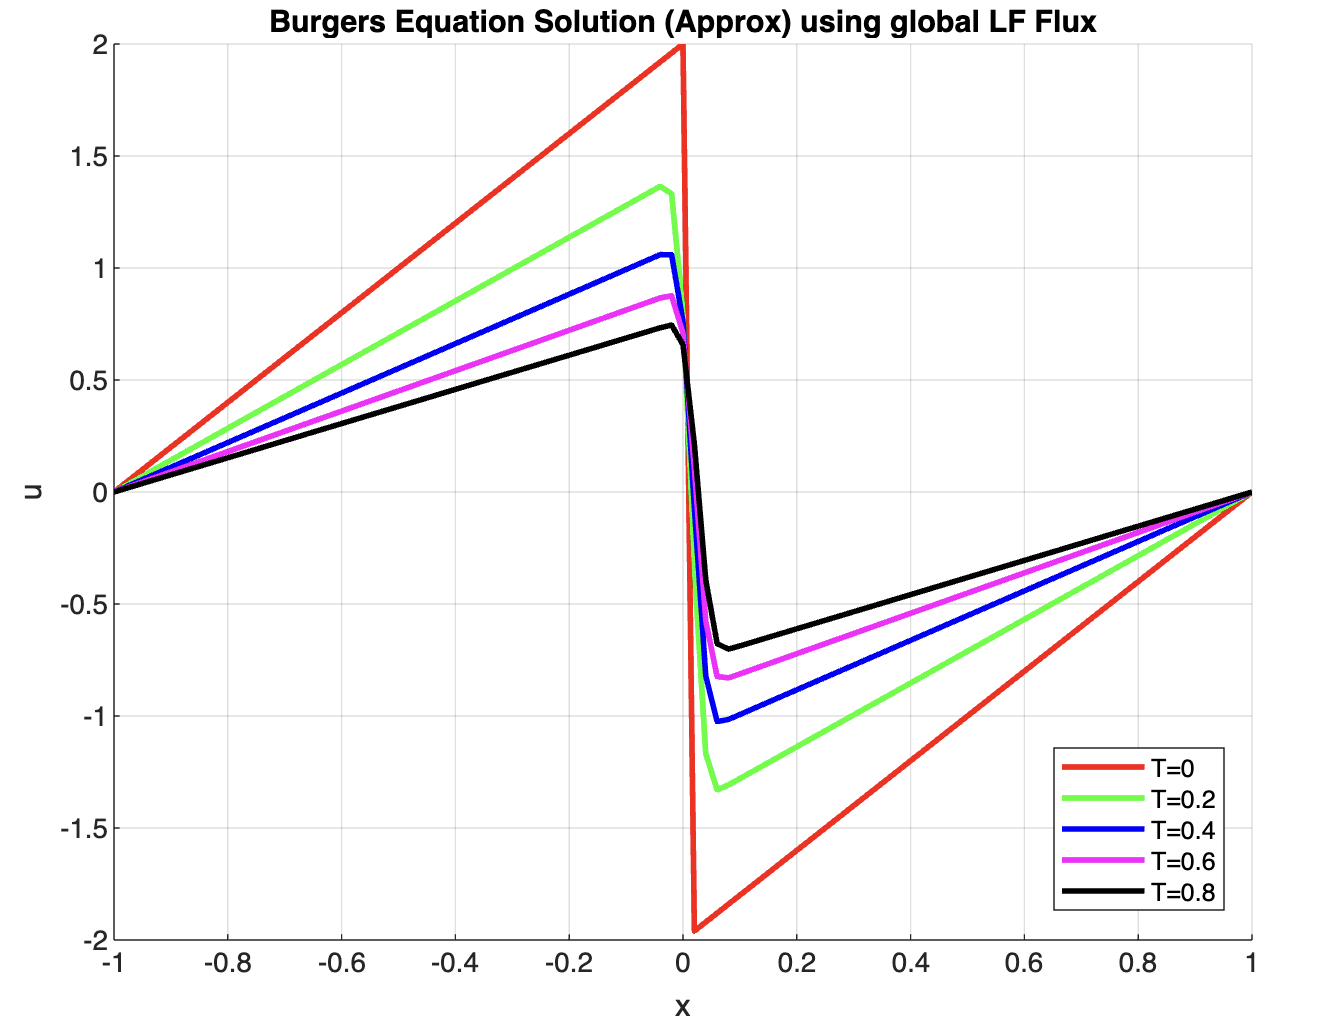
\includegraphics[scale=0.4]{./figures/q6-triangular-global.png}
    \caption{Solving the Burgers equation with a global flux approximate method and triangular initial conditions.}
\end{figure}
Observing the graphs, we see that they mostly look the same. Using the approximate vs the exact methods we note they retain much of the same shape. However in the global setting, we observe more deviation from the true u at the extremes as opposed to the local and exact method. Additionally in the local setting the discontinuity is not as well captured compared to the global and exact methods.
\end{solution}


